\documentclass[11pt,letterpaper]{article}
\usepackage{fullpage}
\usepackage[top=1.5cm, bottom=3.5cm, left=1.5cm, right=1.5cm]{geometry}
\usepackage{amsmath,amsthm,amsfonts,amssymb,amscd}
\usepackage{french}
\usepackage[utf8]{inputenc}
\usepackage[T1]{fontenc}
\usepackage{lastpage}
\usepackage{enumerate}
\usepackage{fancyhdr}
\usepackage{mathrsfs}
\usepackage{xcolor}

\usepackage{graphics} %inclusion de figures
\usepackage{graphicx} %inclusion de figures

\usepackage{sidecap}
\sidecaptionvpos{figure}{c}
\usepackage{listings}
\usepackage{hyperref}
\usepackage{numprint}
\usepackage[bottom]{footmisc}
\usepackage[justification=centering]{caption}
\usepackage[french,frenchkw,boxed,ruled,lined]{algorithm2e}
\SetKw{KwDe}{de}
\SetKw{KwOu}{ou}
\SetKw{KwEt}{et}
\SetKw{Kwrenv}{renvoyer}
\SetKwInput{Variables}{Variables}
\SetKwInput{Variable}{Variable}
\usepackage{xifthen}
\usepackage{colortbl}
\definecolor{green}{rgb}{0.0, 0.5, 0.0}
\usepackage{array,multirow}
\usepackage{wrapfig}
\usepackage{bussproofs}
\usepackage{tikz}
\usetikzlibrary{positioning}
\definecolor{processblue}{cmyk}{0.96,0,0,0}

\newcommand{\exo}[1]{\Large \textbf{Exercice \numprint{#1}} \vspace{10px} \normalsize}
\newcommand\tab[1][12pt]{\hspace*{#1}}

\newcommand{\titlebox}[2]{%
\tikzstyle{titlebox}=[rectangle,inner sep=10pt,inner ysep=10pt,draw]%
\tikzstyle{title}=[fill=white]%
%
\bigskip\noindent\begin{tikzpicture}
\node[titlebox] (box){%
    \begin{minipage}{0.94\textwidth}
#2
    \end{minipage}
};
%\draw (box.north west)--(box.north east);
\node[title] at (box.north) {#1};
\end{tikzpicture}\bigskip%
}

% INFOS
\author{Antoine AFFLATET et Jérémie ROUX (L3 Groupe C)}
\title{HLIN608 - Algorithmique du texte - TD SSP}
\date{2019 - 2020}

\setlength{\parindent}{0cm}

\begin{document}

\maketitle

\vspace{30px}

\titlebox{Problème de décision SSP (\textit{Shortest Superstring Problem})}{
\vspace{3px}
\textbf{Entrée :} Un ensemble de mots $\mathcal{F} = \{F_{1}, ..., F_{n}\}$, et un entier strictement positif $K$.\\
\textbf{Question :} Existe-t-il une superséquence $S$ de $\mathcal{F}$ de longueur $\leq K$ telle que chaque mot de $\mathcal{F}$ est un sous-mot de la superséquence $S $ ?
}

\vspace{30px}

\exo{1}\\
On admet \textit{ssp-optimisation}($\mathcal{F}$) une fonction qui en temps polynomial renvoie la longueur de la plus petite superséquence $S $ telle que chaque mot de $\mathcal{F}$ est un sous-mot de $S $ (algorithme polynomial pour le problème d’optimisation).\\

\begin{algorithm}[H]
    \Si{ssp-optimisation($\mathcal{F}$) $> K$}{
        \textbf{renvoyer} $faux$\;
    }
    \textbf{renvoyer} $vrai$\;
    
    \caption{\textit{ssp-decision}($\mathcal{F}$ : ensemble de mots, $K$ : entier) : booléen}
\end{algorithm}

\vspace{10px}

L'\textbf{Algorithme 1} est en temps polynomial $O(1)+O(ssp-optimisation)$ soit $O(ssp-optimisation)$ où $O(ssp-optimisation)$ est la complexité de ssp-optimisation (polynomial). Ainsi le problème d’optimisation est ``au moins aussi difficile'' que le problème de décision qui lui est associé.\\

\vspace{30px}

\underline{Remarque :}\\ 

On admet maintenant \textit{ssp-decision}($\mathcal{F}$,$K$) une fonction qui en temps polynomial renvoie vrai s'il existe une superséquence $S$ de $\mathcal{F}$ de longueur $\leq K$ telle que chaque mot de $\mathcal{F}$ est un sous-mot de la superséquence $S$, faux sinon (algorithme polynomial pour le problème de décision).\\

\begin{algorithm}[H]
\Variables {min, max, mid : entier;}
    $min \gets 0$\;
    $max \gets 0$\;
    $mid \gets 0$\;
    \PourCh{mot $m$ de $\mathcal{F}$}{
        $max \gets max$ $+$ longueur($m$)\;
    }
    \Tq{$min >= max$}{
        $mid \gets (max - min)/2$\;
        \eSi{ssp-decision($\mathcal{F}$,$mid$)}{
            $max \gets mid$\;
        }{
            $min \gets mid + 1$\;
        }
    }
    
    \textbf{renvoyer} $max$\;
    
    \caption{\textit{ssp-optimisation}($\mathcal{F}$ : ensemble de mots) : entier}
\end{algorithm}

\vspace{10px}

L'\textbf{Algorithme 2} étant en temps polynomial $o(n+log(m)*O($\textit{ssp-decision}$))$ où $n$ est le nombre de mots dans $F$, $m$ la somme des tailles des mots de $F$ et $O($\textit{ssp-decision}$)$ la complexité de \textit{ssp-decision} (polynomial). Ainsi, le problème d’optimisation est ``au moins aussi facile'' que le problème de décision.\\

\vspace{20px}

\exo{2}\\

\begin{algorithm}[H]
\Variables {resultat : booléen; 
i, j : entier;}
 $resultat \gets faux$\;
 
        $i \gets 0$\;
       \Tq{$i < taille(S)$ et~  ! $resultat$}{
        $j \gets 0$\;
        \Tq{$j<taille(m)$ et $m[j]=S[i+j]$}{
          $j \gets j + 1$\;
        }
        \Si{$j=taille(m)$}{
            $resultat \gets vrai$\;
        }
        
         $i \gets i + 1$\;
        }
\textbf{renvoyer} $resultat$\;
    
    \caption{\textit{recherche-naive}($m$ : mot, $S$: superséquence) : booléen}
\end{algorithm}

\vspace{10px}

L'algorithme \textit{recherche-naïve} (\textbf{Algorithme 3}) est en $o(s*n)$ où s est est la taille de S (superséquence) et n la taille du mot m; soit $O(n^2)$.\\

\begin{algorithm}[H]
\Variables {trouve : booléen; 
i : entier;}
    $trouve \gets vrai$\;
    $i \gets 0$\;
    \Tq{$trouve$ et $i<n$}{
        $trouve \gets $ \textit{recherche-naive}$(\mathcal{F}[i],S)$\;
        $i \gets i+1$\;
    }
    \textbf{renvoyer} $trouve$\;
    
    \caption{\textit{verif-ssp}($\mathcal{F}$ : ensemble de mots, $n$ : nombre de mots, $S$ : superséquence) : booléen}
\end{algorithm}

\vspace{10px}

L'algorithme \textit{verif-ssp} (\textbf{Algorithme 4}) est en $o(n*O($recherche-naïve$))$ soit $O(n^3)$ où $n$ est le nombre de mots dans $F$. Ainsi, cet algorithme polynomial vérifie si pour une instance donnée du problème et une superchaîne, cette chaîne satisfait le problème de décision.\\

\vspace{10px}

\exo{3}\\

\begin{figure}[h]
    \centering
    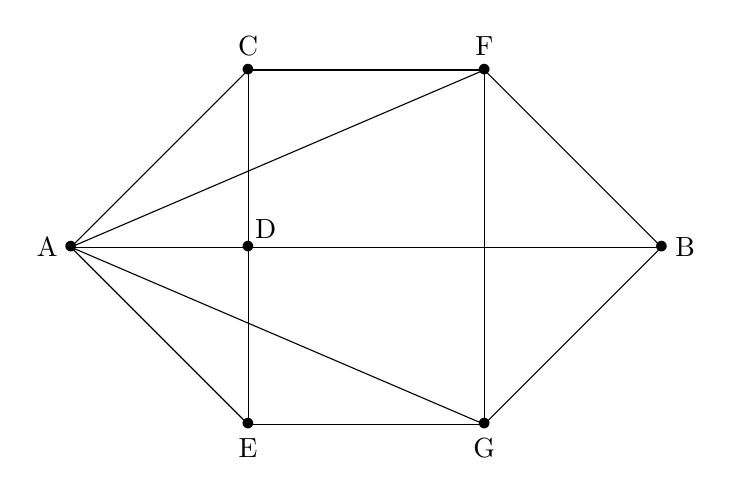
\begin{tikzpicture}[scale=0.75]
    \draw (-0.4,0) node{A};
    \draw (0,0) node{$\bullet$};
    
    \draw (3.3,0.3) node {D};
    \draw (3,0) node{$\bullet$}; 
    
    \draw (3,3.4) node {C};
    \draw (3,3) node{$\bullet$}; 
    
    \draw (7,3.4) node {F};
    \draw (7,3) node{$\bullet$}; 
    
    \draw (10.4,0) node {B};
    \draw (10,0) node{$\bullet$}; 
    
    \draw (7,-3.4) node {G};
    \draw (7,-3) node{$\bullet$}; 
    
    \draw (3,-3.4) node {E};
    \draw (3,-3) node{$\bullet$}; 
    
    \draw (0,0)--(3,3);
    \draw (0,0)--(7,3);
    \draw (0,0)--(10,0);
    \draw (0,0)--(7,-3);
    \draw (0,0)--(3,-3);
    \draw (3,3)--(7,3);
    \draw (7,3)--(10,0);
    \draw (10,0)--(7,-3);
    \draw (3,-3)--(7,-3);
    \draw (3,-3)--(3,3);
    \draw (7,-3)--(7,3);
    \end{tikzpicture}
    \caption{Graphe non-orienté de départ}
\end{figure}

\begin{figure}[h]
    \centering
    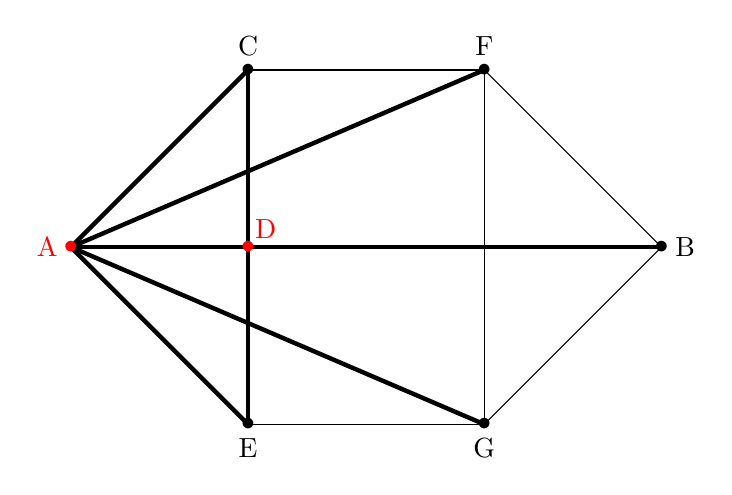
\begin{tikzpicture}[scale=0.75]
    
    \draw (3,3.4) node {C};
    \draw (3,3) node{$\bullet$}; 
    
    \draw (7,3.4) node {F};
    \draw (7,3) node{$\bullet$}; 
    
    \draw (10.4,0) node {B};
    \draw (10,0) node{$\bullet$}; 
    
    \draw (7,-3.4) node {G};
    \draw (7,-3) node{$\bullet$}; 
    
    \draw (3,-3.4) node {E};
    \draw (3,-3) node{$\bullet$}; 
    
    \draw[ultra thick] (0,0)--(3,3);
    \draw[ultra thick] (0,0)--(7,3);
    \draw[ultra thick] (0,0)--(10,0);
    \draw[ultra thick] (0,0)--(7,-3);
    \draw[ultra thick] (0,0)--(3,-3);
    \draw (3,3)--(7,3);
    \draw (7,3)--(10,0);
    \draw (10,0)--(7,-3);
    \draw (3,-3)--(7,-3);
    \draw[ultra thick] (3,-3)--(3,3);
    \draw (7,-3)--(7,3);
    
    \draw[red] (-0.4,0) node{A};
    \draw[red] (0,0) node{$\bullet$};
    
    \draw[red] (3.3,0.3) node {D};
    \draw[red] (3,0) node{$\bullet$}; 
    
    \end{tikzpicture}
    \caption{Exemple d'une couverture minimale pour le graphe de la \textsc{Fig. 1} (taille 2)}
\end{figure}

\vspace{20px}

\titlebox{Problème de décision VERTEX COVER}{
\vspace{3px}
\textbf{Entrée :} Un graphe $G = (V,E)$ et un entier strictement positif $k$.\\
\textbf{Question :} Existe-t-il une couverture des sommets de $G$, notée $C$, de taille $\leq k$ ?
}

\exo{4}\\

\begin{algorithm}[H]
     $\mathcal{F} \gets \{\}$\;
    \PourCh{arête $\{a,b\}$ de $E$}{
        $\mathcal{F} \gets \mathcal{F} \cup \{abab\} \cup \{baba\}$\;
    }
    \vspace{7px}
    \tcc{Calcul de la longueur $H$ de la superchaine $S$ du problème SSP pour laquelle le graphe $G$ admet un vertex-cover de taille $k$, on montrera plus tard que cette dernière vaut 4*|E|+k}
    $H \gets longueurSuperchaine(E,k)$\;
    \vspace{7px}
    \textbf{renvoyer} \textit{ssp-decision}($\mathcal{F}$,$H$)\;
    
    \caption{\textit{VERTEX-COVER}($G = (V,E)$ : graphe, k : entier) : booléen}
\end{algorithm}

\vspace{10px}

En admettant que l'on puisse calculer \textit{ssp-decision} en un temps polynomial et que \textit{longueurSuperchaine} est en $O(1)$, l'\textbf{Algorithme 5} montre une réduction du problème du VERTEX COVER vers le problème SSP (décisionnel) en un temps polynomial $O(n)+O(1)+O(ssp)$. Ainsi la complexité de cet algorithme dépend de la complexité de \textit{ssp-decision} (la transformation étant en temps polynomial O(n)).

\vspace{20px}

\exo{5}\\

L'alphabet considéré est l'ensemble des sommets de la \textsc{Fig. 1}, soit :
$$\Sigma = V = \{a,b,c,d,e,f,g\}$$\\
On étudie le graphe de la \textsc{Fig. 2} qui est un VERTEX COVER du graphe de la \textsc{Fig. 1} :\\
\begin{center}
   \begin{tabular}{|c|c|}
    \hline
    \textbf{Arêtes} & \textbf{Ensemble de chaînes associées}\\
    \hline
    $\{a,c\}$ & $\{acac,caca\}$\\
    \hline
    $\{a,f\}$ & $\{afaf,fafa\}$\\
    \hline
    $\{a,d\}$ & $\{adad,dada\}$\\
    \hline
    $\{a,g\}$ & $\{agag,gaga\}$\\
    \hline
    $\{a,e\}$ & $\{aeae,eaea\}$\\
    \hline
    $\{d,c\}$ & $\{dcdc,cdcd\}$\\
    \hline
    $\{d,e\}$ & $\{dede,eded\}$\\
    \hline
    $\{d,b\}$ & $\{dbdb,bdbd\}$\\
    \hline
\end{tabular} 
\end{center}

\vspace{12px}

On a donc $\mathcal{F}$ qui est l'union des chaines associées aux arêtes du VERTEX COVER, soit :
\vspace{-4px}
$$\mathcal{F} = \{acac,caca,afaf,fafa,adad,dada,agag,gaga,aeae,eaea,dcdc,cdcd,dede,eded,dbdb,bdbd\}$$

\newpage

\exo{6}\\

Soit $m = |E|$ le nombre d'arêtes du graphe du VERTEX COVER, démontrons que :\\
\begin{center}
$G$ a une couverture des sommets de taille $k$\\
$\iff$\\
L'instance transformée de $G$ admet une superchaine de taille $4m + k$.   
\end{center}

\vspace{20px}

\underline{Intuition avec le VERTEX COVER de la \textsc{Fig. 2} :} 
\vspace{-5px}
$$\mathcal{F} = \{acac,caca,afaf,fafa,adad,dada,agag,gaga,aeae,eaea,dcdc,cdcd,dede,eded,dbdb,bdbd\}$$
Par simple concaténation des éléments de $\mathcal{F}$, on obtient une chaîne de longueur $L = 2*4*|E| = 2*4*8 = 64$.\\

\vspace{5px}
Pour chaque arête, on peut associer les deux chaînes entre-elles. On a donc : 
\vspace{-5px}
$$\mathcal{F}_1 = \{acaca,afafa,adada,agaga,aeaea,dcdcd,deded,dbdbd\}$$
Par simple concaténation des éléments de $\mathcal{F}_1$, on obtient une chaîne de longueur $L_1 = 5*|E| = 5*8 = 40$.\\

\vspace{5px}
On peut maintenant regrouper les chaînes qui ont la même première (et dernière) lettre ou dont leur autre forme équivalente respecte cette règle (\{ababa\} $\iff$ \{babab\}). On a donc : 
\vspace{-5px}
$$\mathcal{F}_2 = \{acaca,afafa,adada,agaga,aeaea\} \cup \{dcdcd,deded,dbdbd\}$$

Chaque mot de $\mathcal{F}_2$ a 5 lettres. Si on concatène tous les mots au sein de chaque groupe, on obtient 4 lettres par arête initiale + une lettre représentant le sommet commun à toutes ces arêtes. On a donc $4 * |E|$ lettres + une par groupe avec $k$ groupes, soit $4 * |E| + k$ lettres en tout.\\

Ainsi, on concatène les chaînes qui ont les mêmes premières et dernières lettres. On obtient donc : 
\vspace{-5px}
$$\mathcal{F}_3 = \{acacafafadadagagaeaea,dcdcdededbdbd\}$$

Il ne reste plus qu'à concaténer les mots restants pour obtenir la plus petite superchaine possible ayant comme sous-mots l'ensemble des mots de départ : 
\vspace{-5px}
$$S = acacafafadadagagaeaeadcdcdededbdbd$$
$$longueur(S) = 34 = 4*8+2 = 4*m+k = 4*|E|+k  $$\\

On a donc démontré que $G$ a une couverture des sommets de taille $k$ si et seulement si l'instance transformée de $G$ admet une superchaine de taille $4*m + k$ (avec $m = |E|$). 
\end{document}